\subsection{Consolidamento Requisiti}
\label{consolidamento_requisiti}
In questa fase il gruppo si prepara alla propria presentazione in vista della \textit{Revisione dei Requisiti}.
I componenti si dividono gli argomenti da esporre e descrivono il lavoro svolto nella fase di analisi attraverso delle diapositive.
Inoltre, i membri del \glo{team} si occupano di approfondire individualmente la propria conoscenza delle tecnologie che verranno utilizzate nelle fasi successive.
\textbf{Periodo:} dal 2020-01-14 al 2020-01-18

Le precondizioni sono:
\begin{itemize}
    \item Le \glo{postcondizioni} della fase precedente sono state soddisfatte;
    \item Consegna dei documenti richiesti al proponente.
\end{itemize}
Le postcondizioni sono:
\begin{itemize}
    \item Ultimata preparazione della presentazione da esporre in sede di revisione;
    \item Ogni componente ha studiato le tecnologie necessarie;
\end{itemize}
	
Le attività che vengono svolte sono:
\begin{itemize}
    \item Miglioramento dei documenti e verifica;
    \item Preparazione alla presentazione per la \textit{Revisione dei Requisiti};
    \item Ogni componente dovrà svolgere dello studio autonomo per approfondire le tecnologie necessarie nelle prossime \glo{fasi}.  
\end{itemize}

\subsubsection{Diagramma di Gantt: Consolidamento Requisiti}
\begin{figure}[ht]
    \centering
    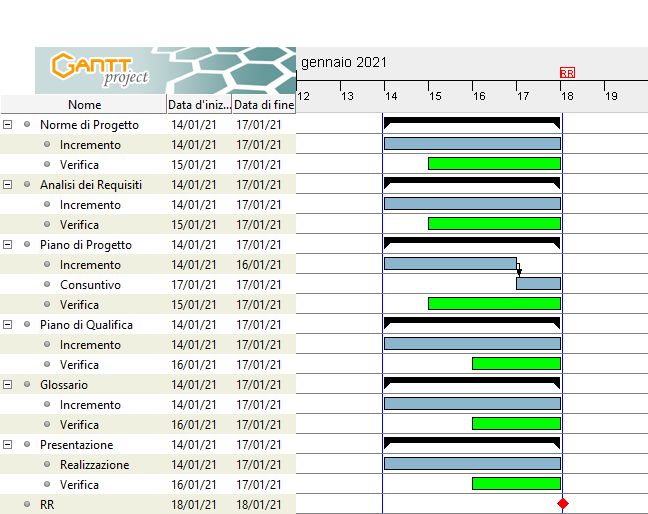
\includegraphics[width=\textwidth]{../../Immagini/Consolidamento.png}
    \caption{Diagramma di Gantt dell'avvitià di Consolidamento dei Requisiti}
\end{figure}
